% rubber : module pdftex
\documentclass{beamer}
%\usetheme{Berkeley}
%\usetheme{Antibes}
\usetheme{CambridgeUS}
\usecolortheme{dolphin}

\title%[SE390] % (optional, only for long titles)
{SE464 Project Deliverable 1 Presentation}
\subtitle{Group 17}
\author[SE2018] % (optional, for multiple authors)
{Software Engineering Class of 2018}
\institute[UW] % (optional)
{
  University of Waterloo
}
\date%[KPT 2004] % (optional)
{September 29, 2016}
\subject{Software Engineering}

%%% BEGIN PREAMBLE

\usepackage{geometry}
% \geometry{screen}
\title{Shots Fired}
\author{scmaier, d2lal, samiskin, wcakeize}

%%% BEGIN DOCUMENT
\begin{document}
\maketitle
\begin{frame}
\frametitle{Project Description}
  \begin{center}
  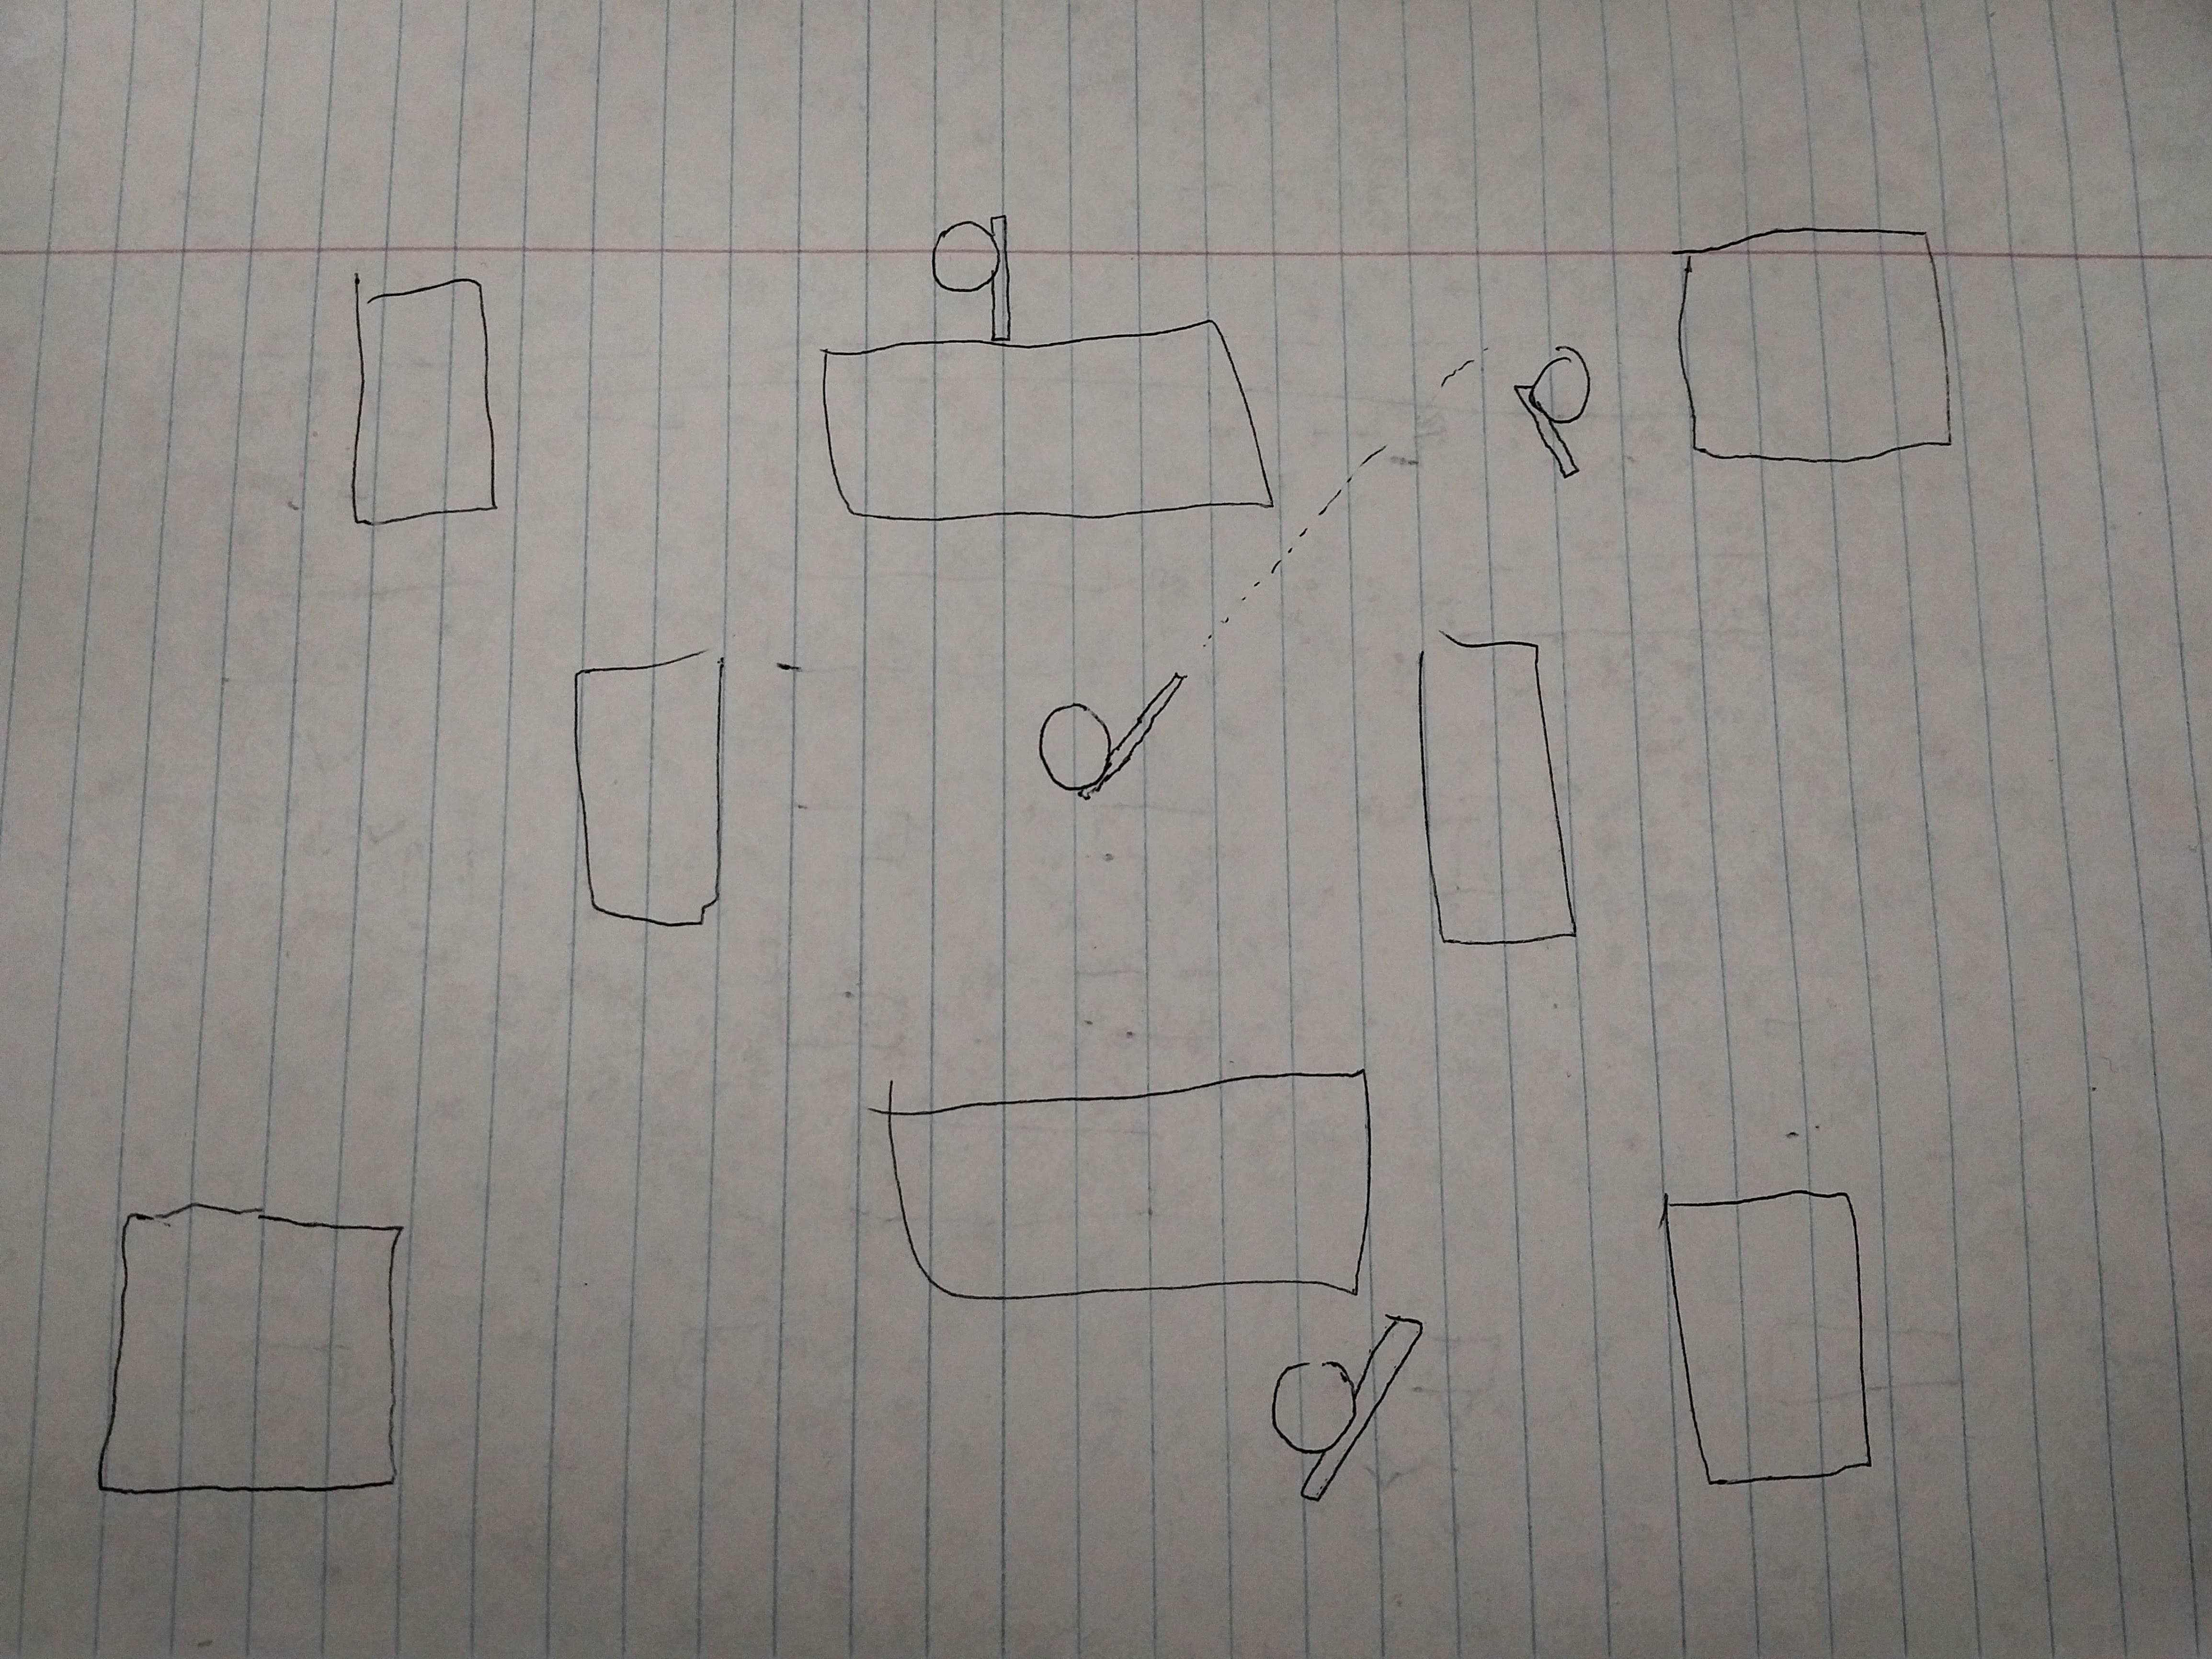
\includegraphics[scale=0.06]{mockup.jpg}
  \end{center}
\end{frame}

\begin{frame}
\frametitle{Design Challenges}
\begin{enumerate}
    \item Creating a game with character interactions, animations, controls, physics, online connections
    \item Synchronizing differences between client and server game states
    \item Running and managing multiple game servers simultaneously
\end{enumerate}
\end{frame}

\begin{frame}
\frametitle{Requirements}
\begin{enumerate}
  \item Top-down arena style 2D shooting game
  \item 2-4 player game played on separate machines connected online
  \item Characters are controlled with Keyboard and Mouse
  \item Can easily join a game with friends (low barrier to entry)
\end{enumerate}
\end{frame}

\end{document}

